\documentclass{article}
\linespread{0.7}
\usepackage[a4paper, margin=3mm, landscape]{geometry}
\usepackage{multicol}
\usepackage{xcolor}
\usepackage{enumitem}
\usepackage{amsmath}
\usepackage{amsfonts}
\usepackage{listings}
\usepackage{soul}
\usepackage{graphicx}

\pdfinfo{
    /Title (cs2103t.pdf)
    /Creator (TeX)
    /Producer (pdfTeX 1.40.0)
    /Author (Vincent Pang)
    /Subject (template)
    /Keywords (cheatsheet, pdf, cs2103t)
}

\graphicspath{ {./img/} }

\pagestyle{empty}
\setcounter{secnumdepth}{0}
\setlength{\columnseprule}{0.25pt}

% Redefine section commands to use less space
\makeatletter
\renewcommand{\section}{\@startsection{section}{1}{0mm}%
    {-1ex plus -.5ex minus -.2ex}%
    {0.5ex plus .2ex}%x
{\normalfont\large\bfseries}}
\renewcommand{\subsection}{\@startsection{subsection}{2}{0mm}%
    {-1explus -.5ex minus -.2ex}%
    {0.5ex plus .2ex}%
{\normalfont\normalsize\bfseries}}
\renewcommand{\subsubsection}{\@startsection{subsubsection}{3}{0mm}%
    {-1ex plus -.5ex minus -.2ex}%
    {1ex plus .2ex}%
{\normalfont\small\bfseries}}%
\makeatother

% Adjust spacing for all itemize/enumerate
\setlength{\leftmargini}{0.5cm}
\setlength{\leftmarginii}{0.5cm}
\setlist[itemize,1]{leftmargin=2mm,labelindent=1mm,labelsep=1mm}
\setlist[itemize,2]{leftmargin=2mm,labelindent=1mm,labelsep=1mm}

% Font
\renewcommand{\familydefault}{\sfdefault}

% Define colors for math formulas
\definecolor{myblue}{cmyk}{1,.72,0,.38}
\everymath\expandafter{\the\everymath \color{myblue}}

% Custom command for keywords
\definecolor{highlight}{RGB}{251,243,218}
\newcommand{\keyword}[2][]{\sethlcolor{highlight}\hl{\textbf{#2}} #1 - }
\newcommand{\ilkeyword}[1]{\sethlcolor{highlight}\hl{\textbf{#1}}}

% Define colors and style for code
\definecolor{codegreen}{rgb}{0,0.6,0}
\definecolor{codegray}{rgb}{0.5,0.5,0.5}
\definecolor{codered}{HTML}{CC241D}
\definecolor{backcolor}{rgb}{0.95,0.95,0.95}
\lstdefinestyle{codestyle}{
    backgroundcolor = \color{backcolor},
    commentstyle = \color{codegray},
    keywordstyle = \color{codered},
    stringstyle = \color{codegreen},
    basicstyle = \ttfamily,
    breakatwhitespace = false,
    showstringspaces = false,
    breaklines = true,
    showtabs = false,
    tabsize = 2
}
\lstset{style = codestyle}

% -----------------------------------------------------------------------
\begin{document}
\begin{multicols*}{4}
\footnotesize

% Title box
\begin{center}
    \fbox{
        \parbox{0.8\linewidth}{
            \centering \textcolor{black}{
                {\Large\textbf{CS2103t}} \\
                \normalsize{Software Engineering 22/23s2 }} \\
                {\footnotesize \textcolor{gray}{github.com/securespider}}
        }
    }
\end{center}

\section{Design}
\subsection{Abstraction}
\begin{itemize}
	\item Establishing a level of complexity and suppress complex details below that level
\end{itemize}
\begin{description}
	\item[Data]{Lower level data items are abstracted and thinking focused on bigger entities}
	\item[Control]{Abstracting details of actual control flow to focus on tasks at higher level}
\end{description}
\subsection{Coupling}
\begin{itemize}
	\item Degree of dependence btw components, classes and methods
	\item Harder maintenance, integration, testing and reuse 
	\item Items are coupled when a change to one requires a change in another
\end{itemize}
\subsection{Cohesion}
\begin{itemize}
	\item How strongly-related and focused various responsibilities of a component are
	\item Keeping related functionalities together
\end{itemize}
\subsection{Separation of concerns principle SoC} 
\begin{itemize}
	\item Achieve better modularity by separating code into distinct sections
	\item each section address separate concerns
	\item Reduce functional overlap btw sections
	\item Reduce coupling and increase cohesion
\end{itemize}
\subsection{Principles}
\begin{description}
	\item[SOLID]
	\begin{description}
		\item[Single Responsiblity Principle]{Classes should only change when responsibilities changes $\approx$ cohesion}
		\item[Open-Closed Principle]{Code entity shld be easy to adapt and reuse w\slash o modifying code entity}
		\begin{itemize}
			\item Using interfaces
		\end{itemize}
		\item[Liskov Substitution Principle]{Derived classes must be substitutable for its base class}
		\item[Interface Segregation Principle]
		\item[Dependency Inversion Principle]
	\end{description}
	\item[Law of Demeter]{Objects shld have limited knowledge and interact with few other objects}
	\item
\end{description}
\section{Models}
\begin{itemize}
	\item Simpler view of a complex entity
\end{itemize}
\subsection{Sequence Diagram}
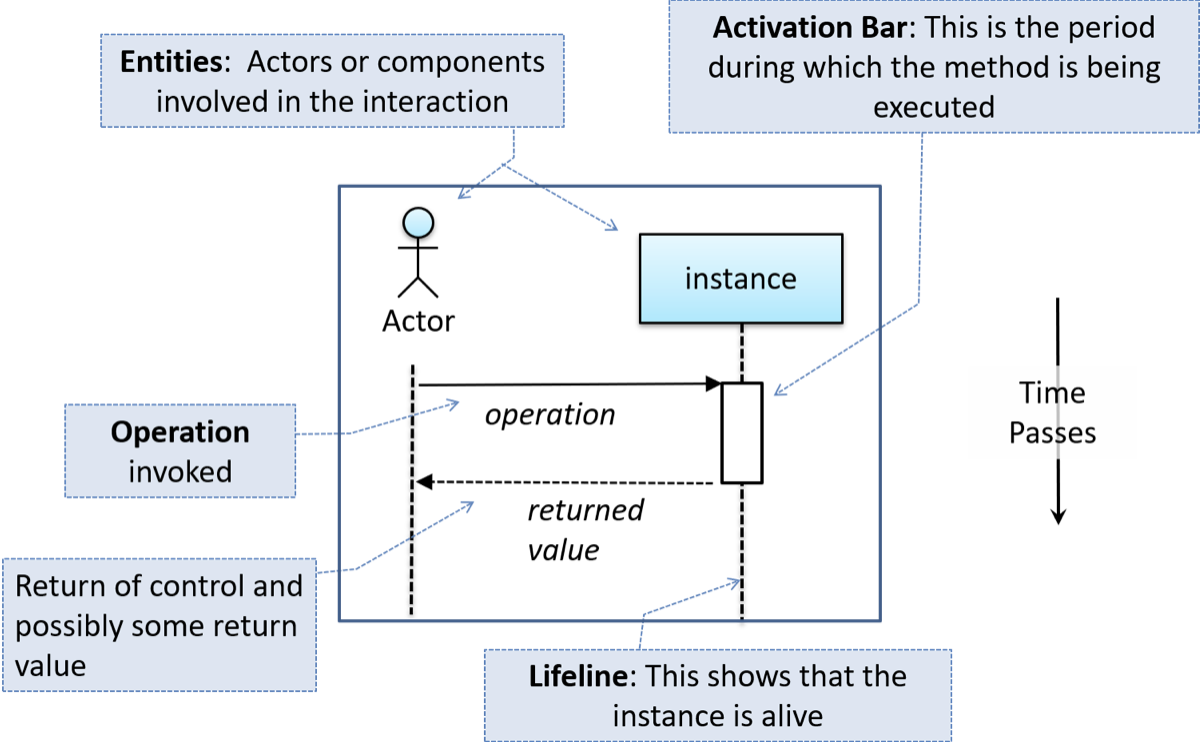
\includegraphics[scale=0.3]{sequence-diagram-basic}
\subsubsection{General}
\begin{itemize}
	\item Stay at the highest level of abstraction instead of the interactions that happen inside each component
	\item Use visual representation
	\begin{itemize}
		\item Associations and navigabilities using lines and arrows connecting classes instead of variables within classes
	\end{itemize}
\end{itemize}
\subsubsection{Arrows}
\begin{itemize}
	\item Must return control to caller
	\item Arrows representing method calls should be solid arrows whereas return should be dashed
	\item Return arrows are optional if it does not result in ambiguities or loss of relevant information
\end{itemize}
\subsubsection{Activation bar}
\begin{itemize}
	\item Activation bar of method cannot start before method call arrives and method cannot remain active after method has returned
	\begin{itemize}
		\item Arrow must start/end at the top/bottom tip of the activation bar
	\end{itemize}
	\item Activation bar should remain unbroken from point method is called until return
	\item These are optional
\end{itemize}
\subsubsection{Entities}
\begin{itemize}
	\item Entities should be in this format `instanceName:Class`
	\item X at the end of the lifeline of an object to show its deletion
	\item Method calls to static that are received by the class itself should have a $<<class>>$ at the top
\end{itemize}
\subsubsection{Paths}
\begin{itemize}
	\item Note that the boxes are not rectangles
	\item Alt boxes may be neither
\end{itemize}
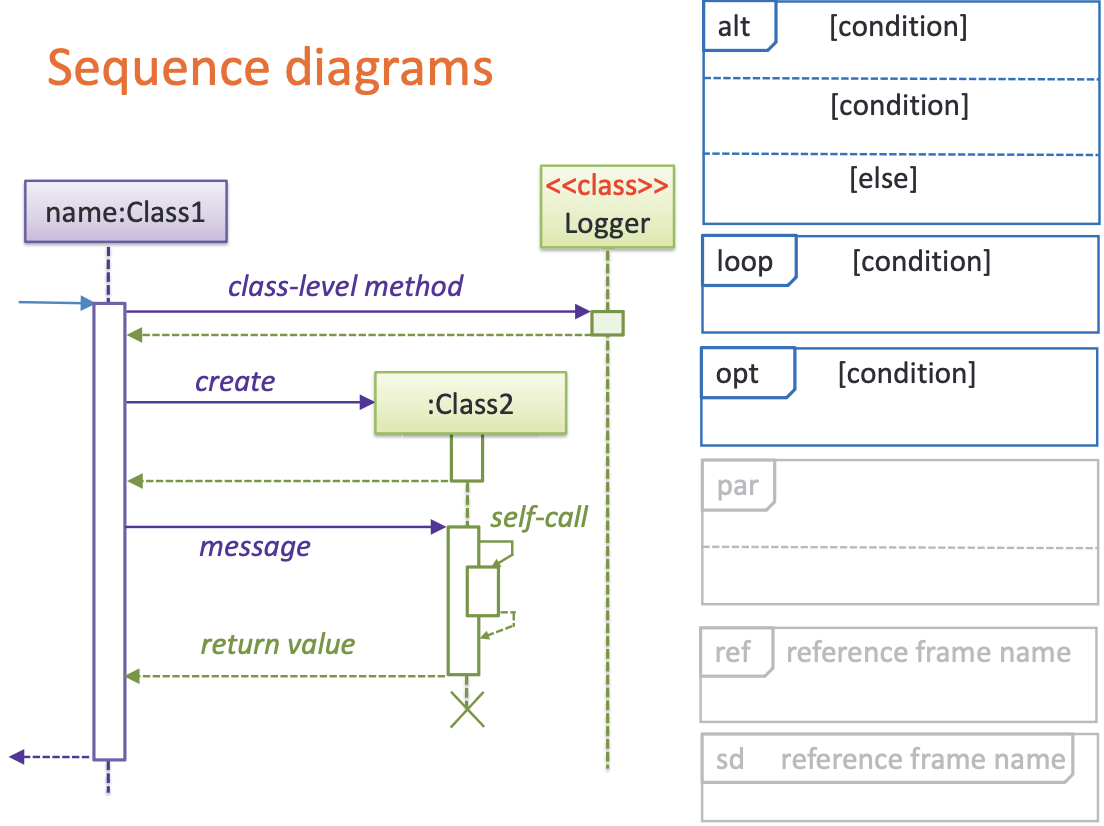
\includegraphics[scale=0.28]{seq-diagram}

\subsection{Activity Diagram}
\begin{itemize}
	\item Consist of start, action, flow/edge
\end{itemize}
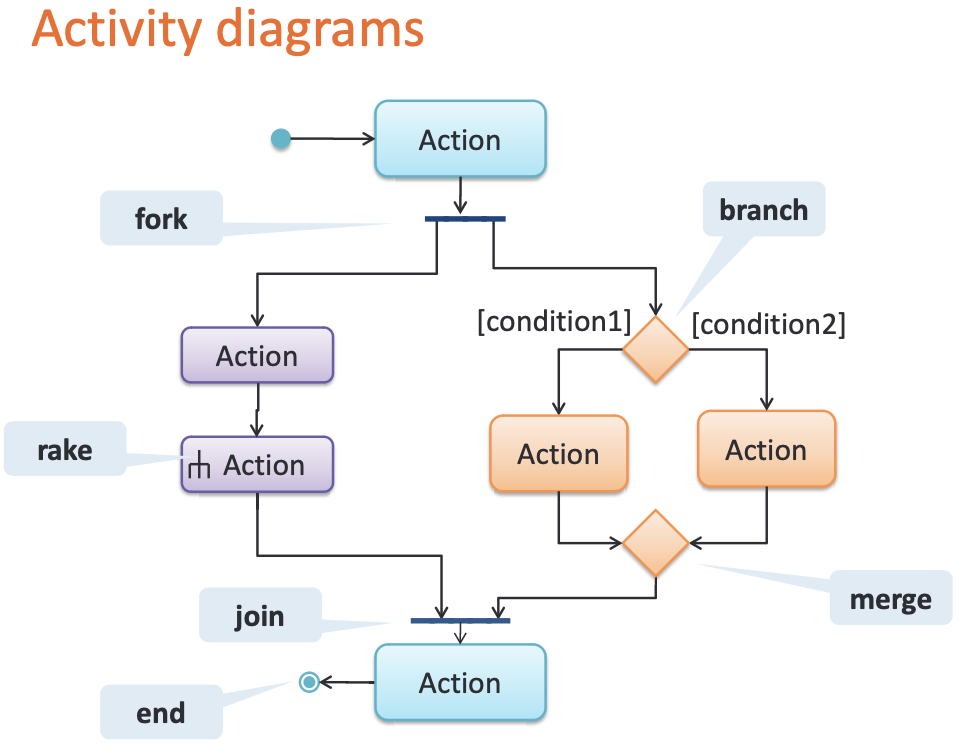
\includegraphics[scale=0.25]{activity-diagram}
\subsubsection{Alternate paths}
\begin{itemize}
	\item Branch node shows start of alternate path with guard conditions
	\begin{itemize}
		\item \keyword{guard}{Boolean condition has to be true for execution to take the path}
	\end{itemize}
	\item Merge node and else conditions can be omited 
	\item Arrows \textbf{MUST} start from the corner
\end{itemize}
\subsubsection{Parallel path}
\begin{itemize}
	\item Execution along all parallel path \textbf{MUST} be complete before execution on outgoing path of join
\end{itemize}
\subsubsection{Rakes}
\begin{itemize}
	\item Indicate that a part of the activity is given as a separate diagram
\end{itemize}
\subsubsection{Swim lanes}
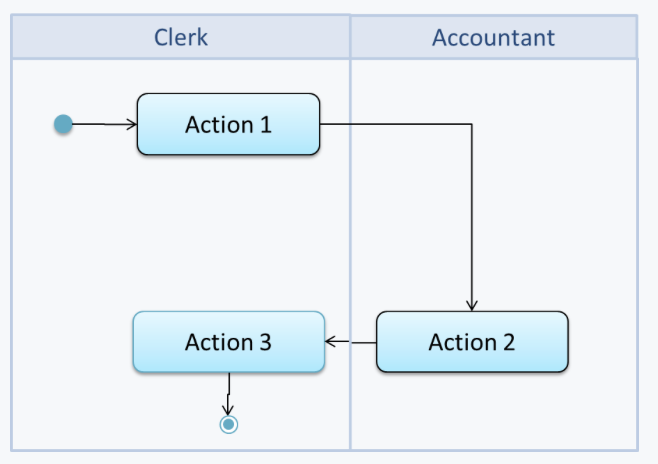
\includegraphics[scale=0.3]{activity-diagram-swimlane}
\begin{itemize}
	\item Partition activity diagram to show who is doing which action
\end{itemize}


\subsection{Class Diagram}
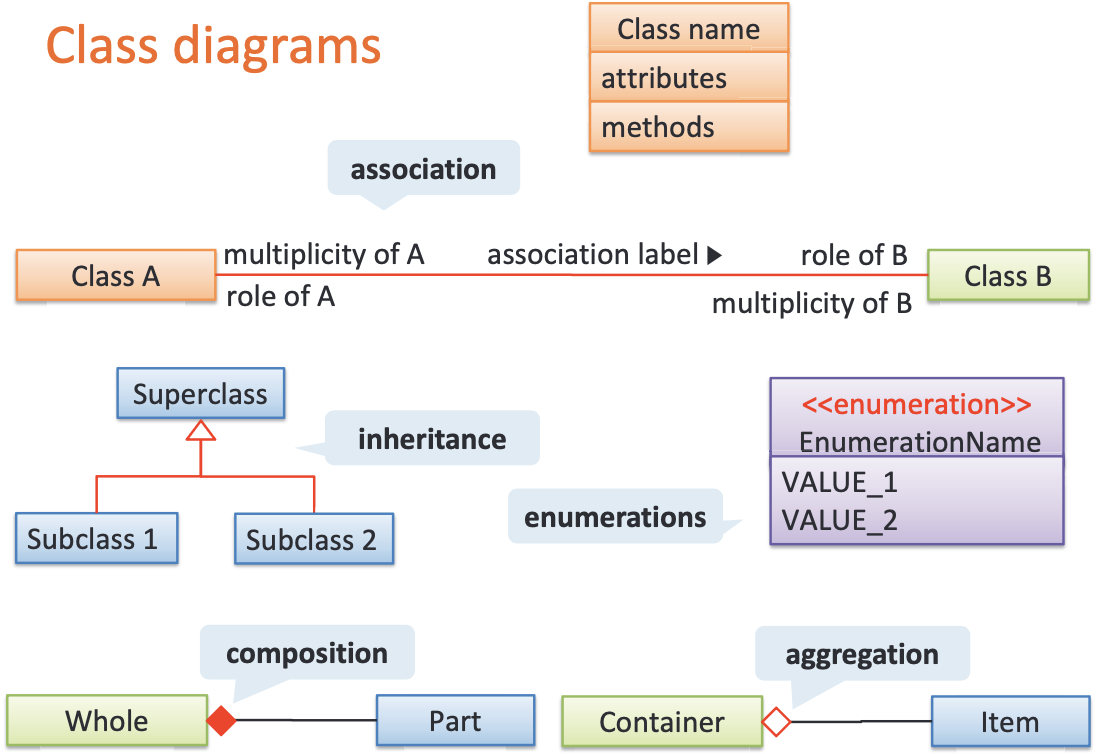
\includegraphics[scale=0.25]{class-diag1}\\
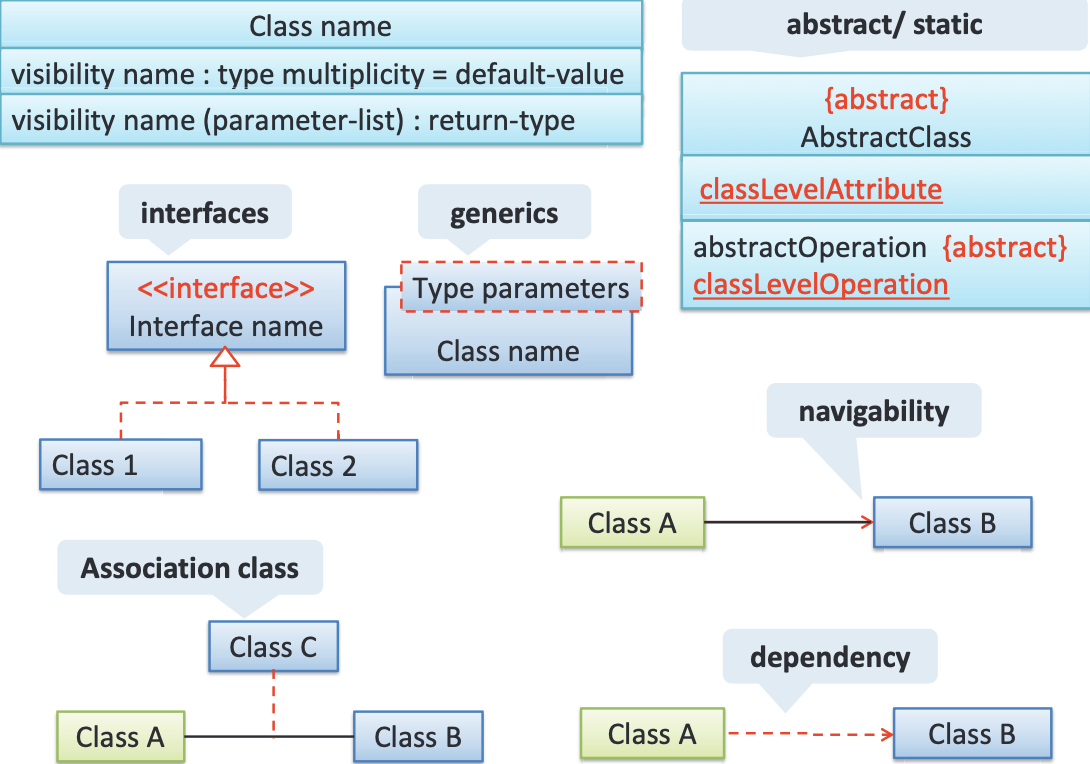
\includegraphics[scale=0.25]{class-diag2}
\subsubsection{Class representation}
\begin{itemize}	
	\item Can contain default values eg. +max:int=0
	\item Operations\slash methods and attributes compartment can be omitted if not important
	\item Underlines denote class-level attributes and methods
	\item Entities can only appear once in a diagram
\end{itemize}
\subsubsection{Visibility}
\begin{description}
	\item[+]{Public}
	\item[-]{Private}
	\item[\#]{Protected}
	\item[\~]{Package private}
\end{description}
\subsubsection{Associations}
\begin{itemize}
	\item Solid line that can have additional decorations like labels, roles, multiplicity and navigability
	\item Multiplicity (eg. m..n - between m and n inclusive, n - exactly n, * - 0 or more objects)
	\begin{itemize}
		\item If class A has multiplicity 2, means 2 objects of A associated to 1 object of other class
	\end{itemize}
	\item \keyword{Navigability}There is a reference from one class to another (can be unidirectional or bidirectional)(optional)
\end{itemize}
\subsubsection{Composition vs Aggregation}
\begin{itemize}
	\item Composition represents strong whole-part relationship 
	\begin{itemize}
		\item If whole is destroyed, parts are destroyed too (eg. Person = whole, name = part)
		\item Commonly used when parts of a big class carved into smaller class for better management
		\item Solid diamond
	\end{itemize}
	\item Aggregation represents container-contained relationship
	\begin{itemize}
		\item Containee object can exist even after container object is deleted (eg. Person in a team)
		\item Hollow diamond
	\end{itemize}
\end{itemize}
\subsubsection{Dependencies vs association}
\begin{description}
	\item[Association]{Object keeping reference of another}
	\item[Dependency]{Class accessing some method/value of another but no association}
\end{description}
\subsubsection{Inheritance}
\begin{itemize}
	\item Abstract classes/methods should either be italicised or with `$\{abstract\}$` keyword
\end{itemize}
\subsubsection{Association Classes}
\begin{itemize}
	\item Represents additional information about association
	\item Should be dotted from the association btw 2 classes
	\item Variables of the 2 classes should not be shown in the association class
\end{itemize}

\subsection{Object Diagram}
\subsubsection{Objects}
\begin{itemize}
	\item Class name and object name (optional) must be underlined in the format `objectName:ClassName`
	\item Should not include methods, only attributes that are relevant to the task
\end{itemize}
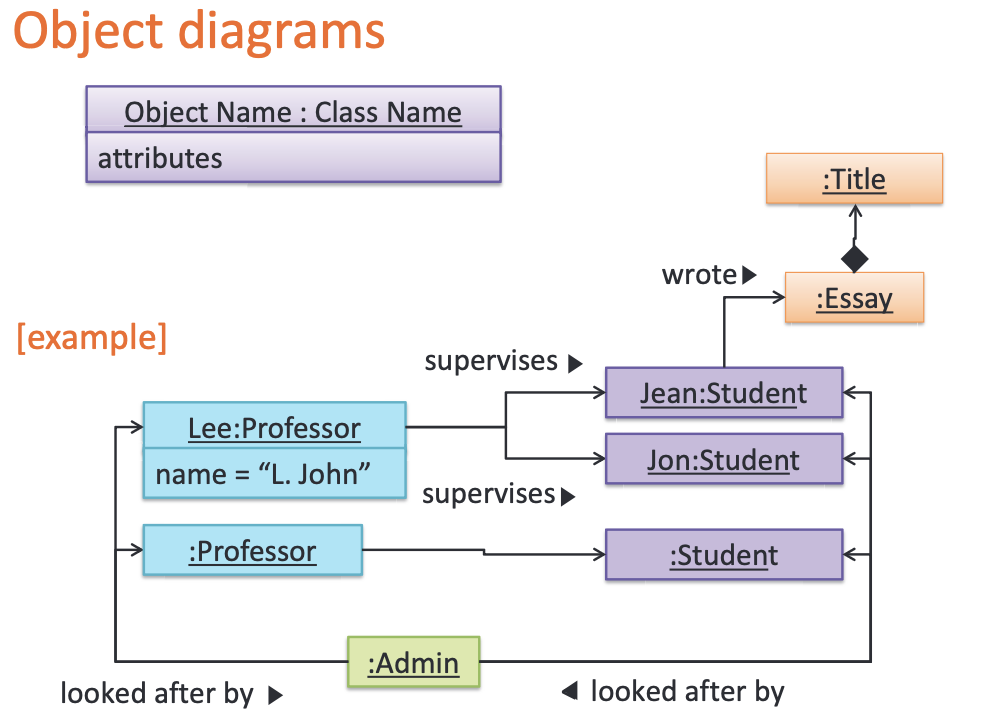
\includegraphics[scale=0.25]{object-diag}

\subsection{Non-functional requirements}
\begin{itemize}
	\item Specify the constraints under which the system is developed and operated
\end{itemize}
\subsubsection{Example requirements}
\begin{description}
	\item[Data]{Size, volatility, persistency (shouldnt be more than 20MB, no crashes, respond within 2s)}
	\item[Environment]{Technical environment which the system would operate in or need to be compatible in (work on 32-bit systems with java installed)}
\end{description}
\subsubsection{Characteristics}
\begin{itemize}
	\item Unambiguous, testable, clear, feasible, atomic (indivisible), necessary, \textbf{implementation-free}
	\item Consistent, non-redundant, complete
\end{itemize}

\subsection{User Stories}
\begin{itemize}
	\item Short simple descriptions of a feature told from perspective of person who wants the capability
	\item Must be in the format `As a \{user type\slash role\} I can \{function\} so that \{benefit\}`
	\begin{itemize}
		\item Benefit can be omitted if obvious
	\end{itemize}
	\item User story should not include any implementation details
\end{itemize}
\subsection{Use cases}
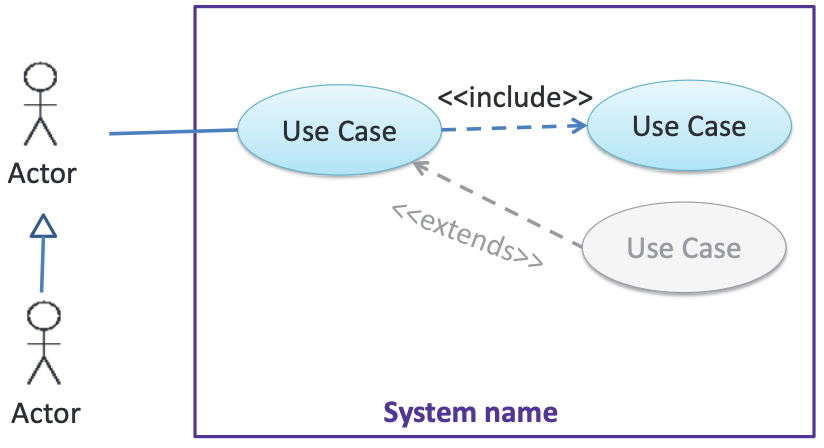
\includegraphics[scale=0.25]{use-case-diag}
\begin{itemize}
	\item Interaction between the user and system for specific functionality of system
	\item Should only describe externally visible behaviour not internal details of a system
	\begin{itemize}
		\item This is wrong: LMS \textit{saves file into cache} and indicate success
	\end{itemize}
	\item Step should give the intention of the actor instead of the mechanics
	\begin{itemize}
		\item UI details should be omitted to give UI designer flexibility in implementation
	\end{itemize}
	\item Can include other use case which \textbf{MUST BE underlined} (inclusions)
\end{itemize}
\subsubsection{Main Success Scenario (MSS)}
\begin{itemize}
	\item Most straightforward interaction for a given use case, assuming nothing goes wrong
	\item Should be self-contained (complete usage scenario)
\end{itemize}
\subsubsection{Extensions}
\begin{itemize}
	\item Add on to the MSS that describes exceptional/alternative flow of events
	\item Extensions should be numerically marked based on when the event may happen
	\begin{itemize}
		\item Extensions marked 3a. happens just after step 3 of MSS (3a1, 3a2...)
		\item Extensions marked *a happens at any step (*a1, *a2...)
		\item Subsequent extensions will be 3b, 4a or *b...
	\end{itemize}
\end{itemize}
\subsubsection{Format}
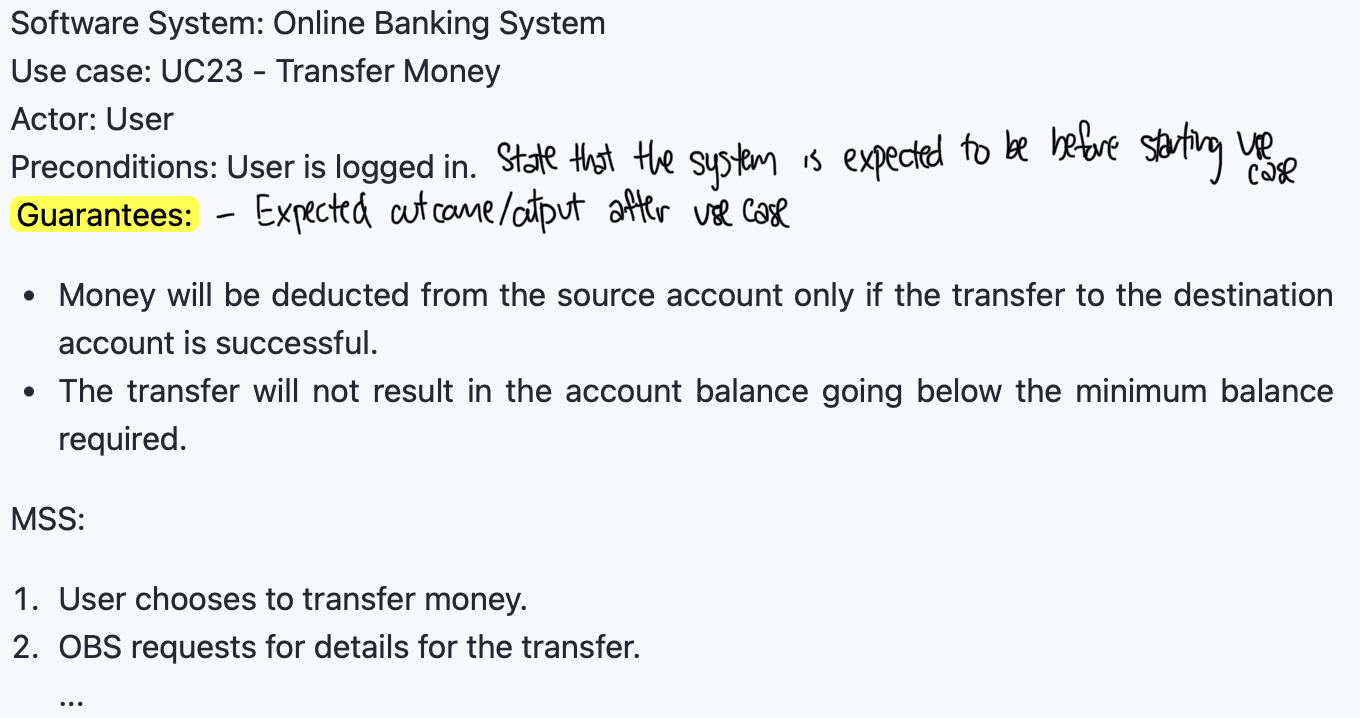
\includegraphics[scale=0.28]{use-case}

\section{Software Architecture}
\begin{itemize}
	\item Software architecture shows overall organization of system as a high-level design
	\item Contains a set of interacting components that fit tog for a specific functionality
	\item Simple and technically viable structure
\end{itemize}
\subsection{Design}
\begin{itemize}
	\item Free-form diagrams with no standard notation
	\item Minimise variety of symbols
	\item Limit use of double-headed arrows to show interaction
\end{itemize}
\subsection{N-tier architectural style}
\begin{itemize}
	\item aka multi-layered, layered
	\item Higher layer make use of services provided by lower 
\end{itemize}
\subsection{Event-driven architectural style}
\begin{itemize}
	\item Flow of application dependent on events from \textit{emitters} and communicated to \textit{consumers} (eg. GUI)
\end{itemize}
\subsection{Other architectural styles}
\begin{description}
	\item[Client-server]
	\item[Transaction processing]{Divides workload of systems into transactions controlled by \textit{dispatcher}}
	\item[Service Oriented]{Combining packages as \textit{programmatically accessible services}}
	\begin{itemize}
		\item Interoperability btw distrbuted system via XML
	\end{itemize}
\end{description}

\section{Software design pattern}
\begin{itemize}
	\item Reusable solution to a commonly recurring problem
\end{itemize}
\subsubsection{Format}
\begin{itemize}
	\item Consist of context, problem, solution, consequences (if-any)
\end{itemize}
\subsection{Singleton}
\begin{description}
	\item[Context]{Classes with \textbf{ONLY ONE} instance}
	\item[Problem]{Normal classes can be instantiated multiple times by calling constructor}
	\item[Solution]{Make constructor private and provide public static method to access single instance}
	\begin{itemize}
		\item Method instantiates instance when executed for the first time
		\item Subsequent calls return single instance of class
	\end{itemize}
	\item[Notation]{$<<Singleton>>$ above the class name in class diagrams}
\end{description}

\subsection{Abstraction occurrence pattern}
\begin{description}
	\item[Context]{Groups of similar entities sharing the same info but slightly different}
	\item[Problem]{Duplication of data which can lead to inconsistencies}
	\item[Solution]{Create an $<<Abstraction>>$ class that holds common information and have unique information in an $<<Occurrence>>$ class}
	\begin{itemize}
		\item eg. Abstraction: BookTitle, Occurence: BookCopy (storing only the serial number)
	\end{itemize}
\end{description}

\subsection{Facade pattern}
\begin{description}
	\item[Context]{Components need to access functionality deep inside other components}
	\item[Problem]{Internal details may be exposed when component is accessed}
	\item[Solution]{Facade class sitting between component internals and users}
	\begin{itemize}
		\item All access to component happens through the facade class
	\end{itemize}
\end{description}

\subsection{Command pattern}
\begin{description}
	\item[Context]{System required to execute number of commands doing specific tasks}
	\item[Problem]{Other objects do not need to know command type to execute commands}
	\item[Solution]{General $<<Command>>$ object that is passed around, stored, executed using polymorphism}
\end{description}

\subsection{Model View Controller (MVC) pattern}
\begin{description}
	\item[Context]{Application supporting storage/retrieval of info, displaying of info and changing stored info from external inputs}
	\item[Problem]{High coupling from the above features}
	\item[Solution]{Decouple data, presentation and control logic of application into 3 different components}
	\begin{description}
		\item[Model]{Stores and maintains data}
		\item[View]{Displays data, interacts with user and pulls data from model}
		\item[Controller]{Detects UI events and executes commands which updates models\slash view if necessary}
	\end{description}
\end{description}

\subsection{Observer pattern}
\begin{description}
	\item[Context]{Multiple objects affected by a change in another object}
	\item[Problem]{Observed object should be decoupled from 'observing' objects}
	\item[Solution]{Force communication through interface known to both parties}
\end{description}

\section{Design approach}
\subsection{Top-down/Bottom-up design}
\begin{description}
	\item[Top-down]{Design high-level before lower level}
	\begin{itemize}
		\item Useful when designing big novel systems where high-level design need to be stable
	\end{itemize}
	\item[Bottom-up]{Design lower-level and put them together to create higher-level}
	\begin{itemize}
		\item Not usually scalable for bigger systems
		\item Useful when designing variation of existing system or repurposing existing components
	\end{itemize}
\end{description}
\subsection{Agile design}
\begin{itemize}
	\item Emergent, not defined up front
	\item Evolves to fulfil new requirements and take advantage of new technologies as appropriate
	\item Some initial architectural modeling
\end{itemize}

\section{Code Quality}
\subsection{Readability}
\subsubsection{Avoid...}
\begin{description}
	\item[Long methods]{Methods should be less than 30 lines of code (LOC)}
	\item[Deep nesting]{Less than 3 levels of indentation}
	\begin{tabbing}
		\=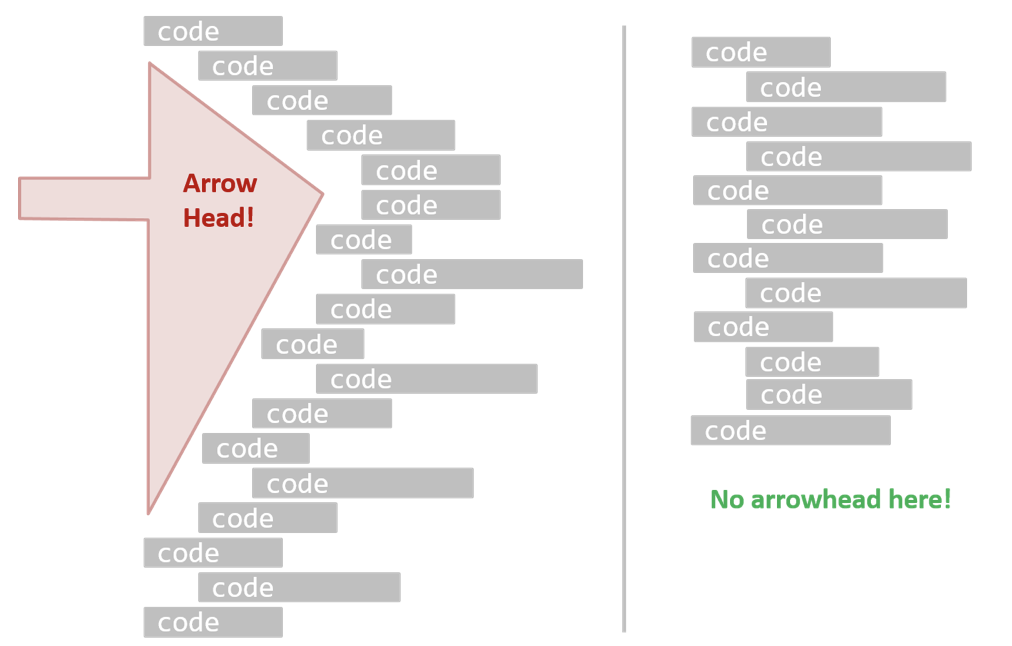
\includegraphics[scale=0.2]{arrowhead-code}
	\end{tabbing}
	\item[Complicated expressions]{Avoid negations and nested parentheses}
	\begin{itemize}
		\item Evaluate complicated expressions in steps with intermediate values
	\end{itemize}
	\item[Magic numbers]{Unexplained numbers should be a named constant}
	\item[Premature Optimization]
	\begin{itemize}
		\item May not know which parts are performance bottlenecks
		\item Complicate code further affecting correctness
		\item Hand-optimization may be slower for compiler to optimise
	\end{itemize}
	\item[Reusing parameters]{Should redeclare local variables with same value as parameter - error prone}
\end{description}
\subsubsection{Should..}
\begin{description}
	\item[Make code obvious]{Explicit type conversions, parentheses to show groupings, enumerations}
	\item[Structure code logically]{Lay out code to adhere logical structure with classes, methods, indentation, linespacing}
	\item[Not trip up reader]{Unused parameters in method, barely similar\slash different things, multiple statements in same line}
	\item[KISS]{Keep things simple (brute-force may be better than complicated}
	\item[SLAP]{Single Level of Abstraction Principle}
	\begin{tabbing}
		\=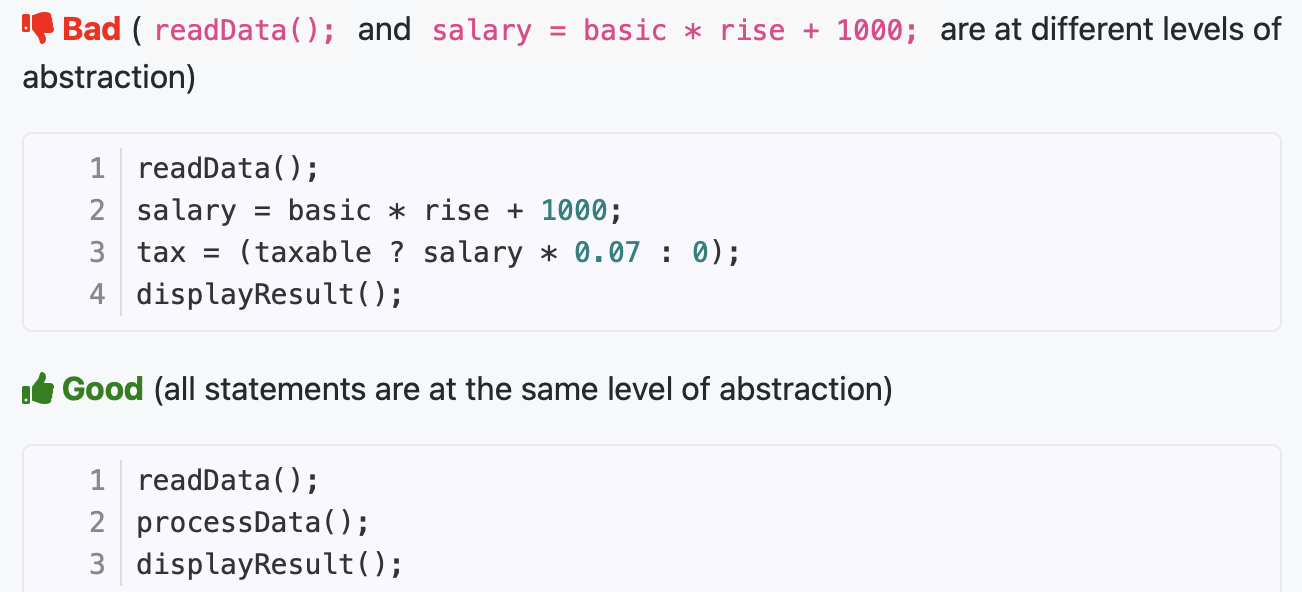
\includegraphics[scale=0.2]{slap-example}
	\end{tabbing}
	\item[Prominent happy path]{Restructure code to make happy path unindented (using guard clauses)}
\end{description}
\subsection{Style guide}
\subsubsection{Naming}
\begin{itemize}
	\item Names representing packages should be in lowercase
	\item Class\slash enum names must be nouns and written in PascalCase
	\item Variable names should be in camelCase
	\item Constant names should be all UPPERCASE using underscore to separate\_words
	\item Methods should be verbs and in camelCase
	\item Boolean variables\slash methods should sound like booleans (eg. isVisible, hasSomething())
	\begin{itemize}
		\item Use prefix such as `is`, `has`, `was`, `can`
	\end{itemize}
	\item Plural form should be used on names representing a collection of objects
	\item Iterator variables can be called i, j, k etc
\end{itemize}
\subsubsection{Layout}
\begin{itemize}
	\item Indentation should be 4 spaces
	\item Line length should be less than 120 char
	\item Indentation for wrapped lines should be 8 spaces more than parent lines (2 tabs)
	\item Egyptian\slash K\&R style eg. while (done) \{
	\item Methods definition: `public void someMethod() throws SomeException \{`
	\item Note there is no indentation for `case` clauses
	\item The explicit \slash\slash Fallthrough comment should be included whenever there is a `case` statement without a break statement
\end{itemize}
\subsubsection{Statements}
\begin{itemize}
	\item Every class should be in some package
	\item Imported classes should always be listed explicitly (no wildcard imports)
	\item Array specifiers should be attached to type not the variables (eg. int[ ] a $>$ int a[ ])
	\item Loops must be wrapped by curly brackets
	\item Conditionals should be placed on separate lines
\end{itemize}
\subsubsection{Javadocs}
\begin{itemize}
	\item Opening \slash ** on a separate lines
	\item First sentence should be a short summary of method
	\begin{itemize}
		\item Starts with strong verbs `returns`, `sends`, `adds`
	\end{itemize}
	\item Subsequent * is aligned with the first *
	\item Space after each *
	\item Empty line between description and parameter section
	\item Punctuation behind each parameter description
	\item No blank line between documentation block and method\slash class
	\item @return can be omitted if method does not return anything
\end{itemize}
\subsubsection{Unsafe shortcuts}
\begin{itemize}
	\item Use default branches (final default and else statements)
	\item Don't recycle variables or parameters
	\item Avoid empty catch blocks
	\item Delete dead code
	\item Minimize scope of variables (limit global variables and keep variable definition within blocks)
	\item Minimize code duplication
\end{itemize}
\subsubsection{Comments}
\begin{itemize}
	\item Do not repeat the obvious
	\item Write to readers
	\item Explain what and why not how
\end{itemize}
\subsubsection{Commits}
\begin{itemize}
	\item Use imperative mood in subject line
	\item Capitalise first letter of subject line
	\item Do not end subject line with period
	\item Separate subject from body with blank line
	\item Body wraps at 72 chars
	\item Blank lines used to separate paragraphs
	\item Explain WHAT, WHY not HOW
	\item Structure for body
	\begin{enumerate}
		\item Current situation
		\item Why it needs to change
		\item What is being done about it
		\item Why it is done that way
		\item Any other relevant info
	\end{enumerate}		
\end{itemize}
\section{Refactoring}
\begin{itemize}
	\item Process of improving a program's internal structure in small steps without modifying its external behaviour
	\item May improve performance and uncover bugs
	\item Refactor $\neq$ rewriting\slash bug fixing
\end{itemize}
\subsection{Consolidate Duplicate Conditional Fragments}
\begin{description}
	\item[Context]{Same fragment of code in all branches of conditional expression}
	\item[Solution]{Move fragment outside the expression}
\end{description}
\subsection{Extract Method}
\begin{description}
	\item[Context]{Code fragments that can be grouped together}
	\item[Solution]{Turn fragment into a method whose name explains purpose of method}
\end{description}

\section{Integration}
\begin{itemize}
	\item Combining parts of software product to form a whole
\end{itemize}
\subsection{Timing}
\begin{description}
	\item[Late and one time]{Integration done when all components are completed}
	\begin{itemize}
		\item Not recommended due to possible component incompatibilities
	\end{itemize}
	\item[Early and frequent]{Evolve each part in parallel in small steps}
\end{description}
\subsection{Extent}
\begin{itemize}
	\item Big bang vs incremental
\end{itemize}
\subsection{Build Automation}
\begin{itemize}
	\item Automating steps of build process using scripts (compiling, linking, packaging)
	\item Help in dependency management
\end{itemize}
\subsubsection{Continuous Integration and Continuous Deployment (CI/CD)}
\begin{description}
	\item[CI]{Integration, building and testing happens automatically after code changes}
	\item[CD]{Changes deployed to end-users as code changes}
\end{description}

\section{Reuse}
\begin{itemize}
	\item Robustness of software system can be enhanced while reducing manpower and time requirement
	\item Reused software may have bugs or not mature enough
\end{itemize}
\subsection{Application Programming Interface (API)}
\begin{itemize}
	\item Specifies the interface for other programs to interact with software component
\end{itemize}
\subsection{Libraries}
\begin{itemize}
	\item Collection of modular code that is general and can be used by other programs
	\item Ensure that library functionality fits your needs
	\item Check license if it allows reuse in the way you use
\end{itemize}
\subsection{Framework}
\begin{itemize}
	\item Reusable implementation of a software providing generic functionality
	\item Customisable to produce a specific application
	\item Similar overall structure and execution flow for specific category of software system
	\item Meant to be customised\slash extended rather than 'as-is'
	\item \keyword{Hollywood principle}{Inversion of control, framework code calls your code}
\end{itemize}
\subsection{Platform}
\begin{itemize}
	\item Runtime environment for application
	\item Bundled with libraries, tools, framework and tech
\end{itemize}

\section{Quality Assurance}
\begin{itemize}
	\item Ensuring software being built has required levels of quality
\end{itemize}
\begin{description}
	\item[Verification]{Requirements implemented correctly}
	\item[Validation]{Requirements are correct}
\end{description}
\subsection{Code reviews}
\begin{itemize}
	\item Systematic examination of code for improvements
	\item PR review, pair prgming, formal inspection
\end{itemize}
\subsection{Formal verification}
\begin{itemize}
	\item Mathematical techniques to prove correctness of prgm
\end{itemize}

\section{Testing}
\begin{itemize}
	\item Executing a set of test cases by specifying input to \textbf{software under test (SUT)} and expected behaviour
	\begin{itemize}
		\item Failure is a mismatch btw expected and actual behaviour
	\end{itemize}
\end{itemize}
\keyword{Testability}{Indication of how easy it is to test SUT depending on design and implementation}
\subsection{Exploratory vs scripted}
\begin{itemize}
	\item \keyword{Scripted}{Writing set of test cases based on expected behaviour and perform testing based on test cases}
	\begin{itemize}
		\item Systematic $\rightarrow$ more bugs detected within sufficient time
	\end{itemize}
	\item \keyword{Exploratory testing}{Devise test cases on the fly based on results of past test cases}
	\begin{itemize}
		\item Simultaneous learning, test design and execution
		\item Dependent on tester experience and intuition
		\item Quick error discovery 
	\end{itemize}
\end{itemize}

\subsection{Regression Testing}
\begin{itemize}
	\item \keyword{Regression}Modification of system that results in unintended and undesirable effects on system 
	\item Re-testing software to detect regression
	\item Test all related components even if tested before
	\item More effective when done frequently after each small change (automation)
\end{itemize}
\subsection{Developer testing}
\begin{itemize}
	\item Testing done by developers as opposed to end-users\slash professionals
	\item Early bug detection $\rightarrow$ easier and cheaper to fix
	\item Do not wait til the end cus of large search space or major reworks
	\item Bugs may hide other bugs
\end{itemize}
\subsection{Unit testing}
\begin{itemize}
	\item Testing individual units to ensure each piece works correctly using Stubs
	\item For each class\slash method separately 
\end{itemize}
\subsubsection{Stubs}
\begin{itemize}
	\item Same interface as the component it replaces but with a simple implementation that is unlikely to have bugs
	\item Should have same responses as component for predetermined inputs
	\item Isolates SUT from dependencies to test unit in isolation
\end{itemize}
\subsection{Integration testing}
\begin{itemize}
	\item Testing whether different parts of the software work together
	\item Aims to discover bugs in the interactions in components\slash "glue code"
\end{itemize}
\subsection{System testing}
\begin{itemize}
	\item Take whole system and test against system specifications
	\item Based on specified external behaviour of system \slash NFRs
\end{itemize}
\subsection{Alpha beta testing}
\begin{itemize}
	\item Deploying to users to test
	\item \keyword{Alpha}Performed under controlled conditions set by SE team
	\item \keyword{Beta}{Given to selected subset of users to test in natural work settings}
\end{itemize}
\subsection{Dogfooding}
\begin{itemize}
	\item SE team use own product IRL to test
\end{itemize}
\subsection{Acceptance testing}
\begin{itemize}
	\item Test system to ensure it meets user requirements
	\item Defined at the beginning of project based on user case specification
\end{itemize}
\subsection{Automation}
\subsubsection{Test Drivers}
\begin{itemize}
	\item Code that 'drives' SUT for purpose of testing
	\item Invokes SUT with test input and verifies if behaviour is as expected (throwing errors)
\end{itemize}
\subsubsection{JUnit}
\begin{itemize}
	\item Tool for automated testing of java programs
\end{itemize}
\subsubsection{GUI testing}
\begin{itemize}
	\item Recommended to move logic out of GUI
	\item Tools: Visual Studio, TestFX, Selenium
\end{itemize}
\subsection{Test Coverage}
\begin{itemize}
	\item Metric used to measure how much testing exercises the code
\end{itemize}
\begin{description}
	\item[Function\slash method coverage]{Based on no. functions executed}
	\item[Statement coverage]{Number of lines of code executed}
	\item[Decision\slash branch coverage]{Based on decision points exercised (if else)}
	\item[Condition coverage]{For all boolean sub-expressions - evaluated to T and F with different test cases}
	\item[Path coverage]{Possible paths through a given part of the code executed}
	\begin{itemize}
		\item More complicated than statement and branch
	\end{itemize}
	\item[Entry\slash exit coverage]{Possible calls to and exits from operations in the SUT}
\end{description}
\subsection{Dependency injection}
\begin{itemize}
	\item 'Injecting' objects to replace current dependencies with different object
	\item Insert stubs to isolate SUT (Used with unit test)
	\begin{itemize}
		\item Polymorphism - stub extends\slash inherits expected class
	\end{itemize}
\end{itemize}
\subsection{Test-Driven Development}
\begin{itemize}
	\item Writing tests before writing SUT thereby defining precise behaviour of SUt using test code
\end{itemize}
\section{Test Case design}
\subsection{Equivalence partition}
\begin{itemize}
	\item Identify groups of inputs that are likely to be processed in the same way
	\item Ensure all partitions are tested, limiting number of inputs from each partition
\end{itemize}
\subsection{Boundary value analysis}
\begin{itemize}
	\item Testing at boundaries of equivalence partitions
	\item Choose 3 values around boundary (before, at, after)
\end{itemize}
\subsection{Combining inputs}
\begin{description}
	\item[All combinations]
	\item[At least once]{3 test case for 3 attributes}
	\item[All pairs]{For any given pair of inputs, all combinations btw them are tested}
	\begin{itemize}
		\item Only need to test pairwise interactions 
		\item Less cases than all combinations strategy
	\end{itemize}
	\item[Random strategy]{Random subset of the other strategies}
\end{description}
\subsubsection{Heuristic}
\begin{itemize}
	\item Each valid input at least once in a positive test case
	\begin{itemize}
		\item Ensure that the valid input results in positive results
	\end{itemize}
	\item No more than 1 invalid input in a test case
	\begin{itemize}
		\item Else would not know which input is the "wrong" one
	\end{itemize}
\end{itemize}
\section{Revision Control (RC)}
\begin{itemize}
	\item Managing multiple versions of a piece of info
	\item Track history for better collaboration
	\item Mistake recovery
\end{itemize}
\subsection{Repository}
\begin{itemize}
	\item Database where meta-data about revision history are stored
	\begin{description}
		\item[Staging]{Specifying files to track and ignore}
		\item[Commit]{Save snapshot of current state of tracked files in RC history}
		\item[Diff]{Compare changes btw 2 points in history}
		\item[Checkout]{Restore state of working directory at a point in the past}
	\end{description}
	\item Commits are uniquely identified by auto-generated hash or tagged
\end{itemize}
\subsubsection{Remote repository}
\begin{itemize}
	\item Repos hosted on remote computers
	\begin{description}
		\item[Clone]{Create a copy of that repo in a location on your computer wit all version history}
		\item[Upstream repo]{Original repo that was cloned}
		\item[Pull]{Receive new commits in second repo from upstream repo}
		\item[Push]{Copy new commits to destination repo with write access and a shared history}
		\item[Fork]{Remote copy of a remote repo without write permissions}
		\item[Pull req]{Mechanism for contributing code to a remote repo with shared history}
	\end{description}
\end{itemize}
\subsection{Branching}
\begin{itemize}
	\item Evolving multiple versions of software in parallel
\end{itemize}
\begin{description}
	\item[RCS]{Revision Control Software}
	\item[Merged]{New commit that maps all changes in other branch to curr}
	\item[Conflicts]{Merging 2 branches that changed the same parts}
	\begin{itemize}
		\item RCS cannot decide changes to keep
		\item Manual conflict resolution
	\end{itemize}
\end{description}
\subsection{CRCS and DRCS}
\begin{description}
	\item[Centralized RCS]{Central remote repo shared by team}
	\begin{itemize}
		\item Members pull and push changes btw local repo and central repo
	\end{itemize}
	\item[Distributed RCS]{Multiple remote repo pulling and pushing in arbitary ways}
\end{description}
\subsection{Forking}
\begin{itemize}
	\item All team members fork main repo and create PR from fork to main repo for changes
\end{itemize}
\section{Software Development Life Cycle}
\begin{itemize}
	\item SDLC provides roadmap for software developers to manage the development effort
	\item Requirements, analysis, design, implementation and testing
\end{itemize}
\subsection{Waterfall/Sequential model}
\begin{itemize}
	\item Models software development as a linear process through the development stages
	\item Each stage of the process should produce some artifacts to be used in the next stage
	\item Useful model when the problem statement is well-understood and stable
	\begin{itemize}
		\item IRL requirements are rarely understood at the beginning and keep changing 
	\end{itemize}
\end{itemize}
\subsection{Iterative models}
\begin{itemize}
	\item Multiple iterations that produces an improved version of the product
	\item Feedback is fed to the next iteration and improved
	\begin{description}
		\item[Breadth-first]{All major components evolved in parallel}
		\item[Depth-first]{Fleshing out individual components before moving to other features\slash components}
	\end{description}
\end{itemize}
\subsection{Agile}
\begin{itemize}
	\item Requirements prioritised based on needs of users and are clarified regularly
	\item Transparency and responsibility sharing among team members
	\item Team works on rough plan and high level design that evolves
\end{itemize}
\subsection{Examples}
\subsubsection{Extreme Programming (XP)}
\begin{itemize}
	\item Priority on customer satisfaction, teamwork
	\begin{itemize}
		\item Delivers software as needed
		\item Respond to changing customer requirements continuously
	\end{itemize}
	\item Communicate with stakeholders (managers, customers and developers) and keep design simple and clean
	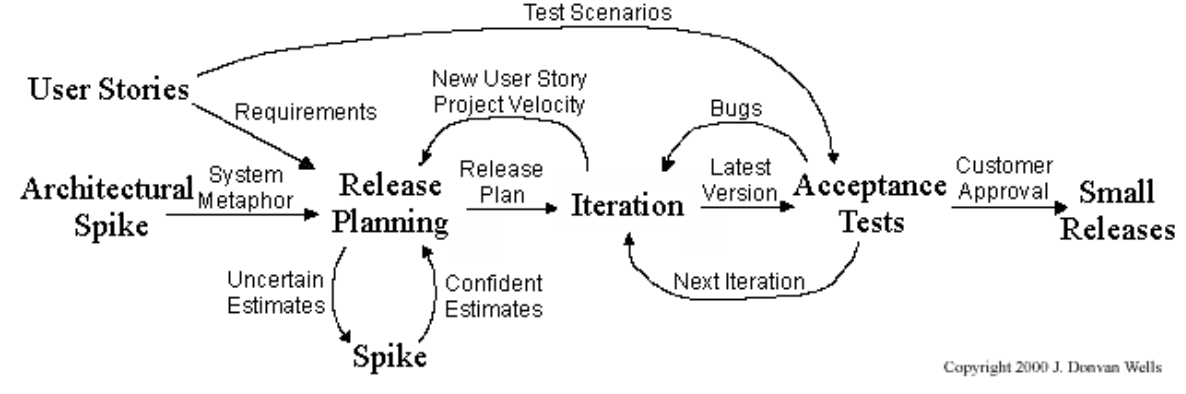
\includegraphics[scale=0.26]{sdlc-xp}
\end{itemize}
\subsubsection{Scrum}
\begin{itemize}
	\item Process skeleton containing sets of practices and roles 
	\begin{itemize}
		\item Scrum master, product owner, team
	\end{itemize}
	\item Divided into iterations called Sprints (timeboxed to specific duration and effort)
	\item Preceded by planning meeting where tasks are identified and commitments made
\end{itemize}
\subsubsection{Unified Process}
\begin{itemize}
	\item Four phases - Inception, Elaboration, Construction and Transition
	\begin{description}
		\item[Inception]{Understand problem and requirements by communication with customer}
		\item[Elaboration]{Refine and expand requirements}
		\item[Construction]{Major implementation effort to support use case}
		\item[Transition]{Ready the system for actual production use}
	\end{description}
	\item Flexible, customisable process model framework
\end{itemize}
\subsubsection{Capability Maturity Model Integration}
\begin{itemize}
	\item Process improvement approach by defining maturity levels for processes
	\item Criteria to determine maturity level of processes
\end{itemize}
\tiny{
\section{Quiz}
\subsection{1}
\begin{itemize}
	\item OOP, Java, Exceptions
\end{itemize}
\subsection{2}
\begin{itemize}
	\item Module\slash SE details, Software Development Life Cycle (SDLC)
	\item Integrated Development Environment (IDE), Revision Control (git terms)
	\item Testing (regression)
\end{itemize}
\subsection{3}
\begin{itemize}
	\item Coding standards, commit messages
	\item Testing (developer and unit (JUnit))
\end{itemize}
\subsection{4}
\begin{itemize}
	\item Model design (Class diagram)
	\item Java varargs, code quality (naming, code reviews, static analysis)
\end{itemize}

\subsection{5}
\begin{itemize}
	\item Object diagram
	\item Requirements (stakeholders, brownfield, NFR, quality, priority)
	\begin{itemize}
		\item Gathering requirements via brainstorming, wireframes
	\end{itemize}
	\item Writing DG (glossary, feature list, user stories)
	\item Code quality (refactoring, naming, comments)
	\item Assertions, streams
\end{itemize}
\subsection{6}
\begin{itemize}
	\item Sequence diagrams
	\item Architecture diagrams (free-form)
\end{itemize}
\subsection{7}
\begin{itemize}
	\item Use cases (MSS)
	\item Design principles, abstraction, coupling, cohesion
	\item Integration and project management
\end{itemize}
\subsection{8}
\begin{itemize}
	\item Diagrams (class, sequence, object)
	\item Testing (types, coverage)
\end{itemize}
\subsection{9}
\begin{itemize}
	\item Diagrams (OODM, Activity)
	\item Principles and SDLC
\end{itemize}
\subsection{10}
\begin{itemize}
	\item Design patterns (singleton, facade, command)
	\item Defensive programming, test case design
\end{itemize}
\subsection{11}
\begin{itemize}
	\item Design patterns (MVC, Observer)
	\item Architecture styles
	\item Testing heuristics, QA (validation vs verification), reuse (platform, frameworks)
\end{itemize}
}
\end{multicols*}
\end{document}
